\documentclass[a4paper,11pt]{paper}
\usepackage{blindtext, graphicx}
\usepackage[utf8]{inputenc}
\usepackage{amsthm}
\usepackage{amsmath}
\usepackage{amssymb}
\usepackage{amsmath}
\usepackage{subfig}
\usepackage{booktabs}
\usepackage{multirow}
\usepackage[table]{xcolor}


\usepackage[firstinits=true,
bibencoding=inputenc,
hyperref=auto,
%style=standard,
refsection=section]{biblatex}
\usepackage{amssymb,amsmath}
\usepackage{tikz}
\newcommand*\circled[1]{\tikz[baseline=(char.base)]{
		\node[shape=circle,draw,inner sep=0.3pt] (char) {#1};}}
\usetikzlibrary{positioning,chains,fit,shapes,calc}
\usepackage{wrapfig}
\usepackage{paralist}

\newcommand{\RNum}[1]{\uppercase\expandafter{\romannumeral #1\relax}}
\usepackage{graphics}

\usepackage{verbatim}
\usepackage{xcolor}
\definecolor{bgcolor}{rgb}{0.99,0.99,0.99}
\definecolor{light-gray}{gray}{0.95}
\usepackage{listings}

 \lstdefinelanguage[OpenCL]{C}[ANSI]{C} 
{  basicstyle=\footnotesize\ttfamily,
	breaklines=true,
	showstringspaces=false,
	numbers=none,
	backgroundcolor=\color{white},
	commentstyle=\color{red},
	keywordstyle=\color{black}\bfseries,
	keywordstyle=[1]\color{black},   % cyan or teal can also be a good choice, use \bfseries for bold
	frame=none,                     % adds a frame around the code
	%xleftmargin=\parindent,
	tabsize=2,                      % sets default tabsize to 2 spaces
	captionpos=b,
	morekeywords={__kernel,kernel,__local,local,__global,global,% 
		__constant,constant,__private,private,% 
		char2,char3,char4,char8,char16,% 
		uchar2,uchar3,uchar4,uchar8,uchar16,% 
		short2,short3,short4,short8,short16,% 
		ushort2,ushort3,ushort4,ushort8,ushort16,% 
		int2,int3,int4,int8,int16,% 
		uint2,uint3,uint4,uint8,uint16,% 
		long2,long3,long4,long8,long16,% 
		ulong2,ulong3,ulong4,ulong8,ulong16,% 
		float2,float3,float4,float8,float16,% 
		image2d_t,image3d_t,sampler_t,event_t,% 
		bool2,bool3,bool4,bool8,bool16,% 
		half2,half3,half4,half8,half16,% 
		quad,quad2,quad3,quad4,quad8,quad16,% 
		complex,imaginary},
	    morekeywords=[1]{               % if you want to add more keywords to the set
		MODELTYPE,
		__CALCL_MODEL_3D,
		MODEL_2D,
		MODEL_3D,
		CALCLcontext,
		CALCLdevice,
		CALCLkernel,
		CALCLManager,
		CALCLmem,
		CALCLModel2D,
		CALCLModel3D,
		CALCLprogram,
		CAL_CUSTOM_NEIGHBORHOOD_2D,
		CAL_CUSTOM_NEIGHBORHOOD_3D,
		CAL_FALSE,
		CALGL_DATA_TYPE_DYNAMIC,
		CALGL_DRAW_MODE_FLAT,
		CALGL_DRAW_MODE_SURFACE,
		CALGL_INFO_BAR_ORIENTATION_VERTICAL,
		CALGL_TYPE_INFO_USE_CURRENT_COLOR,
		CALGL_TYPE_INFO_USE_RED_YELLOW_SCALE,
		CALGL_TYPE_INFO_USE_NO_COLOR,
		CALGL_TYPE_INFO_COLOR_DATA,
		CALGL_TYPE_INFO_NORMAL_DATA,
		CALGL_TYPE_INFO_VERTEX_DATA,
		CALGL_TYPE_INFO_USE_CONST_VALUE,
		CALGL_TYPE_INFO_USE_DEFAULT,
		CALGL_TYPE_INFO_USE_RED_SCALE,
		CALGL_DATA_TYPE_STATIC,
		CALGLRun2D,
		CALGLRun3D,
		CALGLDrawModel2D,
		CALGLDrawModel3D,
		CAL_HEXAGONAL_NEIGHBORHOOD_2D,
		CAL_HEXAGONAL_NEIGHBORHOOD_ALT_2D,
		CAL_MOORE_NEIGHBORHOOD_2D,
		CAL_MOORE_NEIGHBORHOOD_3D,
		CAL_NO_OPT,
		CAL_OPT_ACTIVE_CELLS,
		CAL_RUN_LOOP,
		CAL_SPACE_FLAT,
		CAL_SPACE_TOROIDAL,
		CAL_TRUE,
		CAL_UPDATE_EXPLICIT,
		CAL_UPDATE_IMPLICIT,
		CAL_VON_NEUMANN_NEIGHBORHOOD_2D,
		CAL_VON_NEUMANN_NEIGHBORHOOD_3D,
		calAddActiveCell2D,
		calAddActiveCell3D,
		calAddActiveCellX2D,
		calAddActiveCellX3D,
		calAddElementaryProcess2D,
		calAddElementaryProcess3D,
		calAddSingleLayerSubstate2Db,
		calAddSingleLayerSubstate2Di,
		calAddSingleLayerSubstate2Dr,
		calAddSingleLayerSubstate3Db,
		calAddSingleLayerSubstate3Di,
		calAddSingleLayerSubstate3Dr,
		calAddSubstate2Db,
		calAddSubstate2Di,
		calAddSubstate2Dr,
		calAddSubstate3Db,
		calAddSubstate3Di,
		calAddSubstate3Dr,
		calAddActiveCell2D,
		calAddActiveCellX2D,
		calAddActiveCell3D,
		calAddActiveCellX3D,
		calApplyElementaryProcess2D,
		calApplyElementaryProcess3D,
		CALbyte,
		calclAddActiveCell2D,
		calclAddActiveCellX2D,
		calclAddElementaryProcess2D,
		calclAddElementaryProcess3D,
		calclAddReductionSum2Di,
		calclAddStopConditionFunc2D,
		calclAddStopConditionFunc3D,
		calclAddSteeringFunc2D,
		calclAddSteeringFunc3D,
		calclCreateBuffer,
		calclCreateContext,
		calclCreateManager,
		calCADef2D,
		calCADef3D,
		calclCADef2D,
		calclCADef3D,
		calclFinalizeManager,
		calclFinalize2D,
		calclFinalize3D,
		calclGet2Db,
		calclGet3Db,
		calclGet2Di,
		calclGet3Di,
		calclGet2Dr,
		calclGet3Dr,
		calclGetX2Db,
		calclGetX2Di,
		calclGetX2Dr,
		calclGetX3Db,
		calclGetX3Di,
		calclGetX3Dr,
		calclGetDevice,
		calclGetSum2Di,
		calclGlobalRow,
		calclGlobalColumn,
		calclGlobalSlice,
		calclInitializePlatforms,
		calclInitializeDevices,
		calclLoadProgram2D,
		calclLoadProgram3D,
		calclLocalRow,
		calclLocalColumn,
		calclLocalSlice,
		calclGetKernelFromProgram,
		calclGetRows,
		calclGetColumns,
		calclGetSlices,
		calclgGetByteSubstatesNum,
		calclGetIntSubstatesNum,
		calclGetRealSubstatesNum,
		calclGetCurrentByteSubstates,
		calclGetCurrentIntSubstates,
		calclGetCurrentRealSubstates,
		calclGetNextByteSubstates,
		calclGetNextIntSubstates,
		calclGetNnextRealSubstates,
		calclGetNeighborhood,
		calclGetNeighborhoodID,
		calclGetNeighborhoodSize,
		calclGetBoundaryCondition,
		calclGetPlatformAndDeviceFromStdIn,
		calclRemoveActiveCell2D,
		calclRemoveActiveCell3D,
		calclRun2D,
		calclRun3D,
		calclRunStop,
		calclSetKernelArg2D,
		calclSetKernelArg3D,
		calclThreadCheck2D,
		calclThreadCheck2D,
		calclSet2Db,
		calclSet3Db,
		calclSet2Di,
		calclSet3Di,
		calclSet2Dr,
		calclSet3Dr,
		calclActiveThreadCheck2D,
		calclActiveThreadCheck3D,
		CALDrawModel2D,
		CALDrawModel3D,
		calFinalize2D,
		calFinalize3D,
		calGet2Db,
		calGet2Di,
		calGet2Dr,
		calGet3Db,
		calGet3Di,
		calGet3Dr,
		calGetX2Db,
		calGetX2Di,
		calGetX2Dr,
		calGetX3Db,
		calGetX3Di,
		calGetX3Dr,
		calglAdd2Db,
		calglAdd3Db,
		calglAdd2Di,
		calglAdd3Di,
		calglAdd2Dr,
		calglAdd3Dr,
		calglColor2D,
		calglColor3D,
		calglDefDrawModel2D,
		calglDefDrawModel3D,
		calglDefDrawModelCL2D,
		calglDefDrawModelCL3D,
		calglDisplayDrawJBound2D,
		calglHideDrawJBound2D,
		calglInfoBar2Dr,
		calglInitViewer,
		calglMainLoop2D,
		calglMainLoop3D,
		calglRelativeInfoBar2Dr,
		calglRelativeInfoBar3Dr,
		calglRunCLDef2D,
		calglRunCLDef3D,
		calglSetDisplayStep,
		calglSetHeightOffset2D,
		calglSetHeightOffset3D,
		calInit2Db,
		calInit2Di,
		calInit2Dr,
		calInit3Db,
		calInit3Di,
		calInit3Dr,
		calInitSubstate2Db,
		calInitSubstate2Di,
		calInitSubstate2Dr,
		calInitSubstate3Db,
		calInitSubstate3Di,
		calInitSubstate3Dr,
		CALint,
		calLoadSubstate2Db,
		calLoadSubstate2Di,
		calLoadSubstate2Dr,
		calLoadSubstate3Db,
		calLoadSubstate3Di,
		calLoadSubstate3Dr,
		CALModel2D,
		CALModel3D,
		CALNeighborhood2D,
		CALNeighborhood3D,
		CALOptimization,
		CALParameterb,
		CALParameteri,
		CALParameterr,
		CALreal,
		calRemoveActiveCell2D,
		calRemoveActiveCell3D,
		CALRun2D,
		CALRun3D,
		calRun2D,
		calRun3D,
		calRunAddGlobalTransitionFunc2D,
		calRunAddGlobalTransitionFunc3D,
		calRunAddInitFunc2D,
		calRunAddInitFunc3D,
		calRunAddSteeringFunc2D,
		calRunAddSteeringFunc3D,
		calRunAddStopConditionFunc2D,
		calRunAddStopConditionFunc3D,
		calRunDef2D,
		calRunDef3D,
		calRunInitSimulation2D,
		calRunInitSimulation3D,
		calRunFinalize2D,
		calRunFinalize3D,
		calRunFinalizeSimulation2D,
		calRunFinalizeSimulation3D,
		calSaveSubstate2Db,
		calSaveSubstate2Di,
		calSaveSubstate2Dr,
		calSaveSubstate3Db,
		calSaveSubstate3Di,
		calSaveSubstate3Dr,
		calSet2Db,
		calSet2Di,
		calSet2Dr,
		calSet3Db,
		calSet3Di,
		calSet3Dr,
		calSetX2Db,
		calSetX2Di,
		calSetX2Dr,
		calSetX3Db,
		calSetX3Di,
		calSetX3Dr,
		calSetCurrent2Db,
		calSetCurrent2Di,
		calSetCurrent2Dr,
		calSetCurrent3Db,
		calSetCurrent3Di,
		calSetCurrent3Dr,
		CALSpaceBoundaryCondition,
		CALSubstate2Db,
		CALSubstate2Di,
		CALSubstate2Dr,
		CALSubstate3Db,
		CALSubstate3Di,
		CALSubstate3Dr,
		calUpdateActiveCells2D,
		calUpdateSubstate2Db,
		calUpdateSubstate2Di,
		calUpdateSubstate2Dr,
		calUpdate2D,
		calUpdate3D,
		CALUpdateMode,
	},
}% 

\lstset{language=C}
\lstset{
  basicstyle=\footnotesize\ttfamily,
  breaklines=true,
  showstringspaces=false,
  numbers=none,
  backgroundcolor=\color{white},
  commentstyle=\color{red},
  keywordstyle=\color{black}\bfseries,
  keywordstyle=[1]\color{black},   % cyan or teal can also be a good choice, use \bfseries for bold
  frame=none,                     % adds a frame around the code
  %xleftmargin=\parindent,
  tabsize=2,                      % sets default tabsize to 2 spaces
  captionpos=b,                   % sets the caption-position to bottom
  morekeywords=[1]{               % if you want to add more keywords to the set
    MODELTYPE,
    __CALCL_MODEL_3D,
    MODEL_2D,
    MODEL_3D,
    CALCLcontext,
    CALCLdevice,
    CALCLkernel,
    CALCLManager,
    CALCLmem,
    CALCLModel2D,
    CALCLModel3D,
    CALCLprogram,
    CAL_CUSTOM_NEIGHBORHOOD_2D,
    CAL_CUSTOM_NEIGHBORHOOD_3D,
    CAL_FALSE,
    CALGL_DATA_TYPE_DYNAMIC,
    CALGL_DRAW_MODE_FLAT,
    CALGL_DRAW_MODE_SURFACE,
    CALGL_INFO_BAR_ORIENTATION_VERTICAL,
    CALGL_TYPE_INFO_USE_CURRENT_COLOR,
    CALGL_TYPE_INFO_USE_RED_YELLOW_SCALE,
    CALGL_TYPE_INFO_USE_NO_COLOR,
    CALGL_TYPE_INFO_COLOR_DATA,
    CALGL_TYPE_INFO_NORMAL_DATA,
    CALGL_TYPE_INFO_VERTEX_DATA,
    CALGL_TYPE_INFO_USE_CONST_VALUE,
    CALGL_TYPE_INFO_USE_DEFAULT,
    CALGL_TYPE_INFO_USE_RED_SCALE,
    CALGL_DATA_TYPE_STATIC,
    CALGLRun2D,
    CALGLRun3D,
    CALGLDrawModel2D,
    CALGLDrawModel3D,
    CAL_HEXAGONAL_NEIGHBORHOOD_2D,
    CAL_HEXAGONAL_NEIGHBORHOOD_ALT_2D,
    CAL_MOORE_NEIGHBORHOOD_2D,
    CAL_MOORE_NEIGHBORHOOD_3D,
    CAL_NO_OPT,
    CAL_OPT_ACTIVE_CELLS,
    CAL_RUN_LOOP,
    CAL_SPACE_FLAT,
    CAL_SPACE_TOROIDAL,
    CAL_TRUE,
    CAL_UPDATE_EXPLICIT,
    CAL_UPDATE_IMPLICIT,
    CAL_VON_NEUMANN_NEIGHBORHOOD_2D,
    CAL_VON_NEUMANN_NEIGHBORHOOD_3D,
    calAddActiveCell2D,
    calAddActiveCell3D,
    calAddActiveCellX2D,
    calAddActiveCellX3D,
    calAddElementaryProcess2D,
    calAddElementaryProcess3D,
    calAddSingleLayerSubstate2Db,
    calAddSingleLayerSubstate2Di,
    calAddSingleLayerSubstate2Dr,
    calAddSingleLayerSubstate3Db,
    calAddSingleLayerSubstate3Di,
    calAddSingleLayerSubstate3Dr,
    calAddSubstate2Db,
    calAddSubstate2Di,
    calAddSubstate2Dr,
    calAddSubstate3Db,
    calAddSubstate3Di,
    calAddSubstate3Dr,
    calAddActiveCell2D,
    calAddActiveCellX2D,
    calAddActiveCell3D,
    calAddActiveCellX3D,
    calApplyElementaryProcess2D,
    calApplyElementaryProcess3D,
    CALbyte,
    calclAddActiveCell2D,
    calclAddActiveCellX2D,
    calclAddElementaryProcess2D,
    calclAddElementaryProcess3D,
    calclAddReductionSum2Di,
    calclAddStopConditionFunc2D,
    calclAddStopConditionFunc3D,
    calclAddSteeringFunc2D,
    calclAddSteeringFunc3D,
    calclCreateBuffer,
    calclCreateContext,
    calclCreateManager,
    calCADef2D,
    calCADef3D,
    calclCADef2D,
    calclCADef3D,
    calclFinalizeManager,
    calclFinalize2D,
    calclFinalize3D,
    calclGet2Db,
    calclGet3Db,
    calclGet2Di,
    calclGet3Di,
    calclGet2Dr,
    calclGet3Dr,
    calclGetX2Db,
    calclGetX2Di,
    calclGetX2Dr,
    calclGetX3Db,
    calclGetX3Di,
    calclGetX3Dr,
    calclGetDevice,
    calclGetSum2Di,
    calclGlobalRow,
    calclGlobalColumn,
    calclGlobalSlice,
    calclInitializePlatforms,
    calclInitializeDevices,
    calclLoadProgram2D,
    calclLoadProgram3D,
    calclLocalRow,
    calclLocalColumn,
    calclLocalSlice,
    calclGetKernelFromProgram,
    calclGetRows,
    calclGetColumns,
    calclGetSlices,
    calclgGetByteSubstatesNum,
    calclGetIntSubstatesNum,
    calclGetRealSubstatesNum,
    calclGetCurrentByteSubstates,
    calclGetCurrentIntSubstates,
    calclGetCurrentRealSubstates,
    calclGetNextByteSubstates,
    calclGetNextIntSubstates,
    calclGetNnextRealSubstates,
    calclGetNeighborhood,
    calclGetNeighborhoodID,
    calclGetNeighborhoodSize,
    calclGetBoundaryCondition,
    calclGetPlatformAndDeviceFromStdIn,
    calclRemoveActiveCell2D,
    calclRemoveActiveCell3D,
    calclRun2D,
    calclRun3D,
    calclRunStop,
    calclSetKernelArg2D,
    calclSetKernelArg3D,
    calclThreadCheck2D,
    calclThreadCheck2D,
    calclSet2Db,
    calclSet3Db,
    calclSet2Di,
    calclSet3Di,
    calclSet2Dr,
    calclSet3Dr,
    calclActiveThreadCheck2D,
    calclActiveThreadCheck3D,
    CALDrawModel2D,
    CALDrawModel3D,
    calFinalize2D,
    calFinalize3D,
    calGet2Db,
    calGet2Di,
    calGet2Dr,
    calGet3Db,
    calGet3Di,
    calGet3Dr,
    calGetX2Db,
    calGetX2Di,
    calGetX2Dr,
    calGetX3Db,
    calGetX3Di,
    calGetX3Dr,
    calglAdd2Db,
    calglAdd3Db,
    calglAdd2Di,
    calglAdd3Di,
    calglAdd2Dr,
    calglAdd3Dr,
    calglColor2D,
    calglColor3D,
    calglDefDrawModel2D,
    calglDefDrawModel3D,
    calglDefDrawModelCL2D,
    calglDefDrawModelCL3D,
    calglDisplayDrawJBound2D,
    calglHideDrawJBound2D,
    calglInfoBar2Dr,
    calglInitViewer,
    calglMainLoop2D,
    calglMainLoop3D,
    calglRelativeInfoBar2Dr,
    calglRelativeInfoBar3Dr,
    calglRunCLDef2D,
    calglRunCLDef3D,
    calglSetDisplayStep,
    calglSetHeightOffset2D,
    calglSetHeightOffset3D,
    calInit2Db,
    calInit2Di,
    calInit2Dr,
    calInit3Db,
    calInit3Di,
    calInit3Dr,
    calInitSubstate2Db,
    calInitSubstate2Di,
    calInitSubstate2Dr,
    calInitSubstate3Db,
    calInitSubstate3Di,
    calInitSubstate3Dr,
    CALint,
    calLoadSubstate2Db,
    calLoadSubstate2Di,
    calLoadSubstate2Dr,
    calLoadSubstate3Db,
    calLoadSubstate3Di,
    calLoadSubstate3Dr,
    CALModel2D,
    CALModel3D,
    CALNeighborhood2D,
    CALNeighborhood3D,
    CALOptimization,
    CALParameterb,
    CALParameteri,
    CALParameterr,
    CALreal,
    calRemoveActiveCell2D,
    calRemoveActiveCell3D,
    CALRun2D,
    CALRun3D,
    calRun2D,
    calRun3D,
    calRunAddGlobalTransitionFunc2D,
    calRunAddGlobalTransitionFunc3D,
    calRunAddInitFunc2D,
    calRunAddInitFunc3D,
    calRunAddSteeringFunc2D,
    calRunAddSteeringFunc3D,
    calRunAddStopConditionFunc2D,
    calRunAddStopConditionFunc3D,
    calRunDef2D,
    calRunDef3D,
    calRunInitSimulation2D,
    calRunInitSimulation3D,
    calRunFinalize2D,
    calRunFinalize3D,
    calRunFinalizeSimulation2D,
    calRunFinalizeSimulation3D,
    calSaveSubstate2Db,
    calSaveSubstate2Di,
    calSaveSubstate2Dr,
    calSaveSubstate3Db,
    calSaveSubstate3Di,
    calSaveSubstate3Dr,
    calSet2Db,
    calSet2Di,
    calSet2Dr,
    calSet3Db,
    calSet3Di,
    calSet3Dr,
    calSetX2Db,
    calSetX2Di,
    calSetX2Dr,
    calSetX3Db,
    calSetX3Di,
    calSetX3Dr,
    calSetCurrent2Db,
    calSetCurrent2Di,
    calSetCurrent2Dr,
    calSetCurrent3Db,
    calSetCurrent3Di,
    calSetCurrent3Dr,
    CALSpaceBoundaryCondition,
    CALSubstate2Db,
    CALSubstate2Di,
    CALSubstate2Dr,
    CALSubstate3Db,
    CALSubstate3Di,
    CALSubstate3Dr,
    calUpdateActiveCells2D,
    calUpdateSubstate2Db,
    calUpdateSubstate2Di,
    calUpdateSubstate2Dr,
    calUpdate2D,
    calUpdate3D,
    CALUpdateMode,
    }
}



  \let\oldemptyset\emptyset
\let\emptyset\varnothing
\newtheorem{mydef}{Definition}
\renewcommand{\floatpagefraction}{.72}
\begin{document}
	\title{Relazione Finale - Dottorato di Ricerca in Matematica e
		Informatica - \RNum{30} ciclo}
	\author{
		Davide Spataro \\
		Dipartimento di Matematica e Informatica\\
		Università della Calabria\\
		Via Ponte P. Bucci Rende 87036, \underline{Italia}
	}
	
	
	
	\maketitle
	 

	
	\begin{abstract}
		Durante gli ultimi decenni, il modo in cui applicazioni di calcolo scientifico sono progettate e implementate ed eseguite è radicalmente cambiato. Questo è vero specialmente nei campi della data-analytics, e visualizzazione. Una delle ragioni principali è che le dimensioni dei problemi che vengono trattati dagli scienziati sono molto maggiori e perchè la quantità di dati disponibili ha allargato lo spettro delle possibili applicazioni del calcolo ad ambiti che non erano prevedibili fino a qualche tempo fa.
		Nell'ambito del calcolo scientifico, della modellazione e simulazione in modo particolare, calcolatori paralleli sono usati per ottenere soluzioni approssimate ad equazioni differenziali che descrivono i sistemi fisici che si vogliono studiare in modo rigoroso, come ad esempio le equazionei di \textit{Maxwell} che sono alla base dell'elettromagnetismo classico, o quelle di \textit{Navier-Stokes} per la fluidodinamica.L'approccionclassico, basato sul calcolo differenziale, spesso non riesce a trovare soluzioni analitiche per questi problemi, rendendo necessario soluzioni numeriche approssimate.
		Queste possono esser ottenute utilizzando diversi metodi che sono stati proposti durante gli anni, come il metodo degli elementi finiti, dei volumi finiti o quello delle differenza finite. Quando domini di grandi dimensioni sono considerati, la quantità di calcolo è tale che l'adozione di grandi macchine parallele è assolutamente necessaria. La programmazione di tale macchine è notoriamente complessa, emolte ore lavoro  sono richieste per la scrittura di solver efficienti che siano eseguibili su grandi cluster. Per questo motivo il lavoro finale di tesi è incentrato alla creazione di un'astrazione di programmazione e di una runtime library per l'implementazione di modelli numerici su griglia regolare e che siano eseguibili su clusters di hardware eterogeneo: dalla workstation/laptop, al clusters di CPU/GPUs. Il risultato di questo lavoro è in \texttt{OpenCAL}, che definisce ed implementa un domain specific language per la definizione di una classe di modelli numerici e il loro deployment su macchine parallele. I dettagli architetturali della macchina sono nascosti al programmatore che  con poco sforzo può ottenere diverse versioni del modello numerico: seriale, multi-core, single-GPU, multi-GPU, o cluster di GPU. I risultati ottenuti mostrano che il framework sviluppato è in grado di produrre applicazioni parallele efficienti ed al tempo stesso di ridurre gli sforzi di programmazione necessari per la loro scrittura.


	\end{abstract}
	\newpage
	\tableofcontents

\part{Attività formative e di ricerca -  \RNum{1} anno}
\section{Corsi e Seminari }
	\begin{tabular}{ p{6cm}  l c }
	\toprule
	\rowcolor{gray!65}	
	\textbf{Denominazione} & \textbf{Docente} & \textbf{Periodo}  \\
		\rowcolor{gray!15}	
	SAT-Based Problem Solving & \textit{Joao Marques-Silva} &  Febbraio, 10-12,
	2015 \\
	  \rowcolor{gray!35}
	Mathematical consequences of the existence of very large 
	infinite cardinal numbers & \textit{Joan Bagaria i Pigrau} &  Marzo, 12,
	2015	 \\
		\rowcolor{gray!15}	
	The Identification and Analysis of
	Genomic Transposable Elements & \textit{John Karro} & Giugno, 5, 2015 \\ 
		\rowcolor{gray!35}	
	 Programming GPUs with CUDA & \textit{Manuel Ujaldon} &
	Giugno, 9-11, 2015 \\  
		\rowcolor{gray!15}	
	Descent, CG and Newton Methods On the Quasi-Wolfe Conditions for Self-Scaling Quasi-Newton Methods  & \textit{Mehiddin Al-Baali} &  Luglio,
	1-2, 2015\\
		\rowcolor{gray!35}	 	   
	Congestion Games   & \textit{Angelo Fanelli} &  Gennaio, 22,
	2015 \\
	  
	\bottomrule
\end{tabular}

\section{Partecipazione a  Conferenze}

\begin{itemize}
	\item PDP-2015- Parallel,Distributed and Network-based Processing - Turku,
	Finlandia - 3-6 Marzo 2015
\end{itemize}


\section{Co-supervisione Tesi}
\begin{itemize}
	\item Laurea Magistrale in Informatica - Rahmat Hidayat - \textit{Multi-agent system with multiple groups modelling of bird flocking on GPGPU}.
\end{itemize}

\section{Articoli e Libri Studiati}
\subsubsection{GPGPU and Fluid Simulation}
\begin{itemize}
	\item  Jos Stam-\textit{Flows on Surfaces of Arbitrary Topology}
	\item Jos Stam, \textit{Stable Fluids}
	\item Martin Guay, Fabrice Colin, Richard Egli. \textit{Simple and Fast
		Fluids. GPU Pro, A.K. Peters,Ltd., 2011, GPU Pro, pp.433-444}
	\item Crane, Llamas, Tariq - GPU Gems 3, Real-Time Simulation and Rendering
	of fluids
	\item Mark Harris - GPU Gems,  Fast Fluid Dynamics Simulation on the GPU
	\item Ali Khajeh-Saeedand J. Blair Perot - Computational FluidDynamics
	Simulations using Many Graphics Processors
	\item Stephen Wolfram - Cellular Automaton Fluids: Basic Theory - Journal
	of Statistical Physics
	\item S. Pratap Vanka, Aaron F. Shinn - Computational Fluid
	Dynamics using GPU: Challenge and Opportunities - Proceedings of the ASME
	2011 International Mechanical Engineering Congress \& Exposition IMECE-2011
	\item Pier Luca Lanzi - Accurate real-time fluid dynamics
	using\textit{ Smoothed-Particle Hydrodynamics} and \textit{CUDA}
	\item Yaroslav D. Sergeyev, Higher order numerical differentiation on the
	Infinity Computer, Optimization Letters, pp 575-585
	\item Yaroslav D. Sergeyev,Solving ordinary differential equations on the
	Infinity Computerby working with infinitesimals numerically, Journal of Applied Mathematics and
	Computation (2013)
	\item Markus Billeter et al. Efficient Stream Compaction on Wide SIMD
	Many-Core Architectures
	\item D.M. Hughes, InK-Compact: In kernel Stream Compaction and Its
	Application to Multi-kernel Data Visualization on GPGPU
\end{itemize}

\subsubsection{Termination Problem - Linear Ranking Function}
\begin{itemize}
	\item Roberto Bagnara, Fred Mesnard - Eventual Linear Ranking Functions 
	\item Jan Leike, Matthias Heizmann - Ranking Templates for Linear Loops
	\item Jan Leike - Ranking Function Synthesis for Linear Lasso Programs
	\item Amir M. Ben-Amram - The Hardness of Finding Linear Ranking Functions for
	Lasso Programs
	\item Amir M. Ben-Amram - Mortality of Iterated Piecewise Affine Functions
	over the Integers:  Decidability and Complexity
	\item Amir M. Ben-Amram, Samir Genaim, Abu Naser Masud - On the Termination of
	Integer Loops
	\item Amir M. Ben-Amram, Samir Genaim - Ranking Functions for
	Linear-Constraint Loops
\end{itemize}

\subsubsection{Programmazione Funzionale ed Haskell}
\begin{itemize}
	\item Michael Barr, Charles Wells - Category Theory for Computing Science
	\item Benjamin C. Pierce - A taste of category theory for computer scientists
	\item Simon Marlow - Parallel and Concurrent Programming in Haskell
	\item Simon Peyton Jones, Satnam Singh - A Tutorial on Parallel and
	Concurrent Programming in Haskell - Lecture Notes from Advanced Functional Programming Summer School 2008
\end{itemize}

\subsection{Pubblicazioni}
\begin{itemize}
	\item Alessio De Rango, Mauizio Macr\'i, Davide Spataro, Donato D'Ambrosio and
	William Spataro, \textbf{Efficient Lava Flows Simulations with OpenCL: A
		preliminary application for Civil Defence Purposes}, \emph{Proceedings of
		The10th International Conference on P2P, Parallel, Grid, Cloud and Internet
		Computing, November 4-6, 2015, Krakow, Poland}
	
	\item Filippone G., Spataro W., D'Ambrosio D., Spataro D., 
	Marocco D.,Trunfio G.A., \textbf{CUDA Dynamic Active Thread List Strategy 
		to Accelerate Debris Flow Simulations} \emph{Proceedings of The 2015 International Conference on Parallel, 
		Distributed and Network-Based Processing (PDP)}, Turku, Finland, pp 330-338.
	
	\item Spataro D., D'Ambrosio D., Filippone G., Spataro W., \textbf{The new
		SCIARA-fv3 numerical model and acceleration by GPGPU strategies}
	\emph{International Journal of High Performance and Applications}.
	
	\item Hidayat R., Spataro D., D’Ambrosio D., Spataro W., \textbf{GPU Ac-
		celerated Modeling of Multi-Agent System with Multiple
		Group for Birds Flocking}, \emph{Parallel, Distributed and Network-
		Based Processing (PDP) 2016, accepted}
	\item Hidayat R., Spataro D., D’Ambrosio D., Spataro W., \textbf{Massive
		Parallel Modeling of Birds Flocking on Multi-Agent Sys-
		tem with Multiple Group}, \emph{IEEE Computing in Science and
		Engineering, Discrete Modeling and Simulation Tools, submitted}
\end{itemize}
\section{Attività Di Ricerca}
Il mio percorso di ricerca segue due filoni principali:
\subsection{Calcolo, Simulazione, Visualizzazione e Programmazione Funzionale
	parallela}
Nel contesto del calcolo parallelo la mia attività di ricerca si occupa di
investigare tecniche ed algoritmi innovativi per la simulazione di fenomeno
naturali attraverso macchine parallele ed in particolare utilizzando la GPGPU
programming. Forte enfasi è data ad una classe ampia di problemi la cui
formulazione matematica è basata su equazioni differenziali e le cui
soluzioni numeriche efficienti sono ottenibili mediante decomposizioni a griglia
(Finite element method - \textbf{FEM} -, Finite Volume Method - \textbf{FVM}
-).



\subsection{Stream Compaction}
Ho studiato e sviluppato  un approccio efficiente al problema della stream compaction su processori
grafici di nuova generazione che hanno introdotto le primitive hardware di
ballotting intra-warps.

La stream compaction/reduction è intuitivamente l'operazione di
rimozione, da una collezione, di elementi che non soddisfano un dato
criterio.

Più nel dettaglio, data una lista di elementi  $A_0..A_{N-1}$ di $N$ elementi
ed un predicato $p:A \mapsto \{True,False\}$, il risultato dell'operazione di
stream compaction di $A$ sotto $p$ è $B=\{x \in A \;|\; p(x)=\ True\}$. 
Spesso, nelle applicazioni reali è sufficiente riordinare $A$ tale che gli
elementi validi siano raggruppati. 

La stream compaction è parte fondamentale dell'implementazione
efficiente di molti algoritmi paralleli dove strutture dati sparse di grandi
dimensioni possono essere  difficili da processare, come ad esempio  in
algoritmi di parallel breadht tree traversing, ray tracing, AC, etc.,
e possono portare ad un degrado prestazionale in temini di tempi
d'esecuzione ed efficienza parallela\footnote{Definita come $E=\frac{S}{N}
	$ con $S=\frac{T_1}{T_N}$ ed $N$ il numero di processori utilizzati.}.
L'implementazione seriale è banale mentre quella parallela richiede uno sforzo maggiore, specialmente su
architettura SIMT (single instruction multiple thread) dove è richiesto un
ulteriore step intermedio, la prefix sum (o scan). 
\begin{mydef}{Prefix Scan}
	
	Dato un operatore binario associativo  $\diamond$, una collezione di $N$
	elementi $V_{0 \ldots {N-1}}$ ed un elemento identità $I$ per $\diamond$
	allora la prefix scan è la collezione $P$ definita come segue:
	\[
	P= \{I,V_0,(V_0 \diamond V_1),(V_0 \diamond V_1 \diamond V_2) \ldots
	(V_0 \diamond V_1 \diamond \ldots \diamond V_{N-1}) \}
	\]
	
\end{mydef}

\subsubsection{Stream Compaction parallela}\
Supponiamo che $P$ sia il numero di processori ed $N$ la size della
collezione, $N>P$ (nei casi reali $N>>P$) e che l'input stream
sia diviso in substream di size $S$.
L'algoritmo è composto da tre fasi distinte:
\begin{enumerate}
	\item Ogni processore $p_i$ conta in modo indipendente il numero di
	elementi validi nel proprio substream salvandolo in $PC[p_i]$
	\item Viene effettuata un' operazione di prefix sum ($\diamond = +, I=1$)
	su $PC$ producendo l'offset a cui ogni processore scriverà il proprio
	risultato finale $PO[p_i]$.
	\item Ogni processore scrive in modo indipendente il proprio output (gli
	elementi validi) senza interferire con gli altri nella locazione
	$OUT[PO[p_i]]$.
\end{enumerate}


\subsubsection{Stream Compaction on SIMT Hardware}\label{smparallel}
L'hardware  delle moderne GPU è composto di un numero dell'ordine delle decine
di streaming multiprocessors (SMM), che intuitivamente sono un array di processori SIMD a
loro volta composti dalle SIMD lanes, i cosidetti Streaming Processors. Le
nuove architetture hardware NVIDIA contano 16 SMM e 128 SP per SMM per un
totale di oltre 2000 cores.
Ogni SMM esegue il threads a blocchi indivisibili di 32, i warp, all'interno
dei quali ogni thread esege in modo sincrono le stesse istruzioni. SMM non
sono processori scalari e quindi usando lo stesso approccio descritto al
paragrafo \ref{smparallel}, si otterebbero valori di efficienza parallelo
molto bassi a causa del fatto che per ogni SMM verrebbe utilizzato un solo
core (avremmo infatti un altissimo numero di idle SIMD
lanes,$ 16\times(128-1)=2048-16$).

Per ovviare a questo problema ogni fase dell'algoritmo descritto al paragrafo
\ref{smparallel} è stata riadattata per sfruttare al massimo la potenza di
calcolo disponibile, ed in particolare:
\begin{description}
	\item[Phase 1]
	Ogni SMM ha il compito di gestire una porzione dello stream di input, e
	procedendo a gruppi di \textbf{warpSize} calcola, tramite un operazione di
	reduce il numero di elementi validi nella
	porzione dell'input gestita dal SMM.
	\item[Phase 2]
	Output della fase precendente è un array di counter che viene usato durante
	questa fase per calcolare, attraverso l'operazione di prefix sum, l'offset
	di output per ogni SMM.
	\item[Phase 3]
	Questa fase prende in input lo stream da compattare e l'array di offset
	calcolato alla fase precedente e restituisce in output lo stream compattato.
	Utilizza le funzioni di ballotting (introdotte nelle moderne architetture
	GPU) che consentono a i thread di uno stesso warp di comunicare senza
	incorrere in alcun overhead. Intuitivamente computa warp, block a grid
	offset, in modo che ogni thread abbia a disposizione l'esatta locazione di
	output per un elemento valido dello stream di input\footnote{Che ha indice
		di output: offset del thread nel warp sommato a quello del warp nel blocco,
		e quello del blocco nella griglia.}.
\end{description}
I moduli CUDA/C che implementano questa operazione sono liberamente
disponibili al seguente url: \url{https://github.com/knotman90/cuStreamComp}


\subsection{Bird Flock Simulation on GPU}
Ho lavorato ad un simulatore parallelo su GPU per la simulazione di Bird
flocks basato sul modello di proposto da Craig W. Reynolds in 1987. Esso
descrive tre leggi cui ogni agente della simulazione ad ogni step
temporale obbedisce:
\begin{description}
	\item[1: coesione] è il vettore forza diretto verso il centro di massa dello
	stormo 
	\item [2: separazione]  è il vettore forza, che mantiene l'agente ad una
	distanza minima da tutti gli altri boids
	\item [3: allineamento] è la forza che sincronizza i vettori velocità di un
	agente con i suoi vicini
\end{description}

Il sistema, adotta un approccio multi-agents multiple
groups per la modellazione della dinamica degli stormi. Il modello sviluppato
è basato su quello di Reynolds, e lo estende aggiungendo il supporto alla
coesistenza e l'interazione di diverse specie e per la presenza di predatori.
Gli esperimenti condotti mostrano che l'utilizzo della GPGPU in questo ambito ha
garantito un significativo aumento delle performance in termini di speedup
(fino a 700x) confermando la validità di questa tecnologia anche in ambito
multi-agents modeling. 

Questo lavoro ha ispirato il design di una libreria per
agenti autonomi in GPU che verrà sviluppata durante il secondo anno di dottorato.

\subsection{Soluzioni numeriche di ODE e PDE utilizzando Grossone}
Assieme al prof. Ya. D. Sergeyev, basandoci su un suo lavoro che applica il
sistema numerico Grossone, da lui ideato, alla risoluzione di ODE e PDE
abbiamo sviluppato una libreria Haskell per la manipolazione numerica di
equazioni differenziali nel suddetto sistema numerico. Questa sarà uno dei
blocchi costituenti di un solver parallelo a precisione arbitraria.

 \subsection{Termination problem e ranking functions}
L'analisi della terminazione è stata oggetto di numerosi studi negli ultimi
anni, con un conseguente aumento del numero e dell'accuratezza dei tools per
lo studio statico della terminazione di programmi.

Il caso generale, l'halting problem, è indecidibile, ma molte sottoclassi
sono decidibili e ampiamente studiate, come ad esempio quello della
terminazione dei cosidetti loop lineari deterministici. In questo contesto la mia ricerca si occupa di
investigare il ruolo e le proprietà di una particolare classe di funzioni, le
\textbf{multiphase linear ranking functions}, che si sono dimostrate essere un
valido strumento per la dimostrazione della terminazione dei suddetti loop (
si vedano definizioni seguenti). La mia ricerca è orientata all'investigazione di
problemi teorici riguardanti:
\begin{itemize}
	\item L'esistenza di un algoritmo (assieme a soundness e completeness) per
	la sintetizzazione di questo tipo di ranking function sia sui razionali che sugli interi.
	\item L'esistenza di un bound di qualche tipo sul numero di componenti.
	\item Individuazione di sottoclassi di SLC che hanno una RF di questo tipo.
\end{itemize}



\begin{mydef}
	Un single path linear constraint loop  su $n$ variabili $x_1 \ldots x_n$ \`e
	della forma
	
	\[
	while (Bx \leq b); \:\: do \: \;A \begin{pmatrix}x\\x'\end{pmatrix} \leq c
	\] 
	dove $B \in \mathbb{Q}^{m \times n}$, $x,x' \in \mathbb{Q}^n$, $b \in
	\mathbb{Q}^n$, $A \in \mathbb{Q}^{p \times n}$ e $c \in
	\mathbb{Q}^p$. \\ $(Bx \leq b)$ e $A \begin{pmatrix}x\\x'\end{pmatrix} \leq c$
	sono chiamati rispettivamente \textbf{guard} e \textbf{update} del loop.
	Quest'ultimo è \textbf{deterministico} se pu\`o essere riscritto come un sistema
	di uguaglianze ($A \begin{pmatrix}x\\x'\end{pmatrix} = c$).
	Il vettore $\begin{pmatrix}x\\x'\end{pmatrix} \in \mathbb{Q}^{2n}$ vive nello
	spazio delle transizioni del loop. Pi\`u formalmente 
	$\begin{pmatrix}x\\x'\end{pmatrix}$ è una transizione se $x$  soddisfa il guard 
	e $x'$ l' update.
\end{mydef}

\subsubsection{Multiphase ranking function - MPhiRF}

Consideriamo un SLC Q. Una tupla \(<\rho_1,...,\rho_d>\) è una MPHiRF
se per ogni transizione \(\begin{pmatrix}x\\x'\end{pmatrix} \in Q\), \(\exists i \in [1..d]\) tale che:
\begin{enumerate}
	\item $\begin{aligned}[t]
	\rho_j(x)-\rho_j(x') \geq 1, \;\;\forall j \leq i\\
	\end{aligned}$
	\item $\begin{aligned}[t]
	\rho_i(x) \geq 0\\
	\end{aligned}$
	\item $\begin{aligned}[t]
	\rho_j(x)< 0,  \;\;\forall j<i\\
	\end{aligned}$
\end{enumerate}

Intuitivamente esiste una funzione $\rho_1(x)$ che è sempre
decrescente in  Q e quando diventa negativa $\rho_2(x)$ inizia a decrescere,
e quando anch'essa diventa negativa ne esiste un altra che decresce nella stessa
maniera e così via.

Ovviamente tutto ciò \textbf{implica la terminazione del loop}.

Il punto (1) significa che quando una componente inizia a decrescere, lo farà
per sempre.
I punti (2,3) significano che se usiamo la $i$-esima componente per il ranking
di $\begin{pmatrix}x\\x'\end{pmatrix}$, allora tutte le componenti $j<i$ sono
già negative, altrimenti ne avremmo usata una tra quelle per effettuare il ranking di $\begin{pmatrix}x\\x'\end{pmatrix}$
-- perchè sono anch'esse decrescenti.
Si noti come (3) è in qualche modo ridondante perchè avremmo potuto definire la
stessa classe di funzioni prendendo il più piccolo indice $i$ tale che (1,2)
fossero verificati.

Come esempio, consideriamo il seguente loop:
\[while ( x>0 )\: { x'=x+y, y'=y-1 }\]

che ha MPhiRF: \(<y,x>.\)
Tutte le transizioni del tipo $(x,y\geq 0)$ hanno come ranking function
$\rho_1(x)=y$ che è positiva e decrescente $(y-(y-1)) =1 \geq 1$. Quando essa
diventa negative --per le transizioni del tipo $(x,y<0)$--, allora
$\rho_2(x)=x$ è positiva e decrescente $(x - (x-y)) = y \geq 1$.


\part{Attività formative e di ricerca -  \RNum{2} anno}
\section{Corsi e Seminari}
\begin{itemize}
	\item Deep Learning – Theory and Applications in the Natural Sciences - Pierre Baldi - 12/09/2016 , Universtià della Calabria
\end{itemize}


\section{Pubblicazioni}
\begin{itemize}
\item \textit{Davide Spataro, Paola Arcuri, Alessio De Rango, William Spataro, Donato
D’Ambrosio and Alice Mari}, \textbf{TraCCA - A Complex Cellular Automata
based Particle Tracking Framework}, Accepted, 25th Euromicro
International Conference on Parallel, Distributed, and Network-Based
Processing (PDP 2017) San Pietroburgo, Russia (lavoro congiunto con
Ricercatori dell’Università di Edinburgo - UK)

	\item \textit{Donato D’Ambrosio, Alessio De Rango, Marco Oliverio, Davide Spataro,
William Spataro, Rocco Rongo, Giuseppe Mendicino, Alfonso Senatore},
\textbf{The Open Computing Abstraction Layer for Extended Cellular
Automata and the Finite Differences Method}, Submitted to the
ISI/SCOPUS Journal of Parallel and Distributed Computing (ISSN: 0743-
7315)

\item \textit{Andrea Giordano, Alessio De Rango, Davide Spataro, Donato D’Ambrosio,
Gianluigi Folino, William Spataro}, \textbf{Asynchronous execution
of cellular automata: the SciddicaS3-hex case study}, Accepted to
25th Euromicro International Conference on Parallel, Distributed, and
Network-Based Processing (PDP 2017) San Pietroburgo, Russia

\end{itemize}	

\subsection{Partecipazione a  Conferenze}

\begin{itemize}
  \item PDP-2016- Parallel,Distributed and Network-based Processing - Heracklion, Creta,
  Grecia- 17-19 Febbraio  2016
\end{itemize}



\section{Attività di Ricerca}
La mia attività di ricerca svolta durante il secondo anno di dottorato ha riguardato due filoni distinti. Un primo percorso è stato sviluppato durante un periodo di research visiting presso L'università di Edimburgo ed ha riguardato principalmente il settore dei cosiddetti Big-Data e più precisamente la visualizzazione interattiva di grandi moli di dati.
Il secondo filone è stato portato avanti in congiunzione con un altro gruppo di ricercatori presso l'istituto di BioEngineering dell'Università di Edimburgo ed ha riguardato il tracking di particelle a partire da immagini al microscopio.


\subsection{VELaSSCo - Visualization For Extremely Large-Scale Scientific Computing}
\subsubsection{Introduzione}
Ho partecipato attivamente allo sviluppo di \textit{VELaSSCo}, una piattaforma che mira ad essere in grado di rendere possibili le analisi e visualizzazioni di simulazioni dell'ordine dell' exabyte attraverso l'utilizzo di processing in-situ per la data-analytics e GPGPU per la visualizzazione. La piattaforma è sviluppata da un consorzio aziendale ed universitario europeo i cui componenti sono \textit{CIMNE} (Spagna), \textit{SINTEF} (Norvegia), \textit{INRIA} (Francia), Fraunhofer \textit{IGD} (Germania), \textit{Jotne} (Norvegia), \textit{Atos} (spagna), \textit{School of Engineering UEDIN} (Scozia), e finanziato da un progetto europeo di 3.1M. 
L'attività di ricerca è stata portata a termine presso la ``University of Edinburgh", School of Engineering, Infrastructure and Environment, Kings Building EH9 3BF, sotto la supervisione del Prof. Jin Ooi. 
All'interno dell'ecosistema \textit{VELaSSCo} , il mio lavoro di ricerca si è incentrato sul design e sviluppo del modulo di visualizzazione che deve essere in grado di produrre rappresentazioni 3D interattive di modelli dell'ordine del Tera/Exabyte.

\subsubsection{Descrizione della Piattaforma}
\begin{figure}[!htbp]
	\centering
	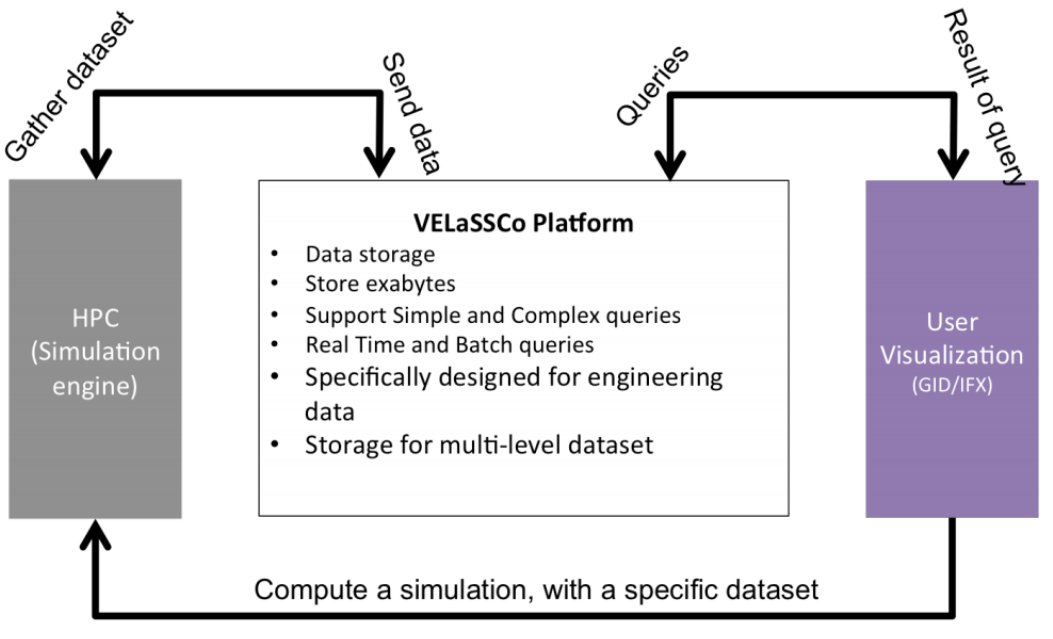
\includegraphics[width=\textwidth]{images/vel}
	\caption{Interazione di \textit{VELaSSCo} con i moduli di calcolo e simulazione e quelli di visualizzazione.}
	\label{fig:vel}
\end{figure}
Il design di \textit{VELaSSCo} (Figura \ref{fig:vel}) è incentrato su tre macro componenti principali.
\begin{description}
	\item [Data Layer] Si occupa dello storage e dell'organizzazione fisica dei dati all'interno della macchina distribuita. E' basato sull'utilizzo di database distribuiti come HBase .
	\item [Data Analytics Layer] Si occupa dell'analisi dei dati. E' implementato seguendo il paradigma map-reduce  ed è ciò che rende la piattaforma estremamente scalabile, estensibile e generale. Moduli analitici esterni scritti da terze parti possono essere facilmente integrati all'interno del sistema per fare fronte alle esigenze analitiche dell'analisi e/o simulazione previste.
	\item [Visualization Layer] 
	Questo modulo ha l'obiettivo di rendere possibile la visualizzazione 2-3/D dei dati e l'interazione con il modulo di analytics.
\end{description}
Il workflow tipico nell'ambito del calcolo scientifico prevede
\begin{inparadesc}
	\item[l'esecuzione] del solver o modello di simulazione in un HPC, il
	\item[salvataggio]  dati su disco ed infine il
	\item[trasferimento] dei dati dall'HPC al client di visualizzazione ed analisi.
\end{inparadesc}
Storicamente un approccio di questo tipo ha avuto successo principalmente perché l'hardware grafico e di calcolo erano completamente separati e differenze tra velocità di calcolo e scrittura su disco erano relativamente piccole.
Tuttavia, dopo l'avvento della GPGPU, la distinzione netta tra HW grafico e
HW di calcolo è stata drasticamente diminuita, ed il divario tra velocità dei processori e quella dei dispositivi di storage permanente è arrivato ad essere di almeno di due ordini di grandezza.
Ad aggravare la situazione di inadeguatezza del workflow tipico vanno ad aggiungersi che l'avvento delle tecnologie che vanno sotto al nome di Big-Data  hanno fatto si che solvers siano in grado di produrre quantità di dati impensabili fino a pochi anni fa (soprattutto nel campo dell'ingegneria e della fisica). 
\begin{figure}[!htbp]
	\centering
	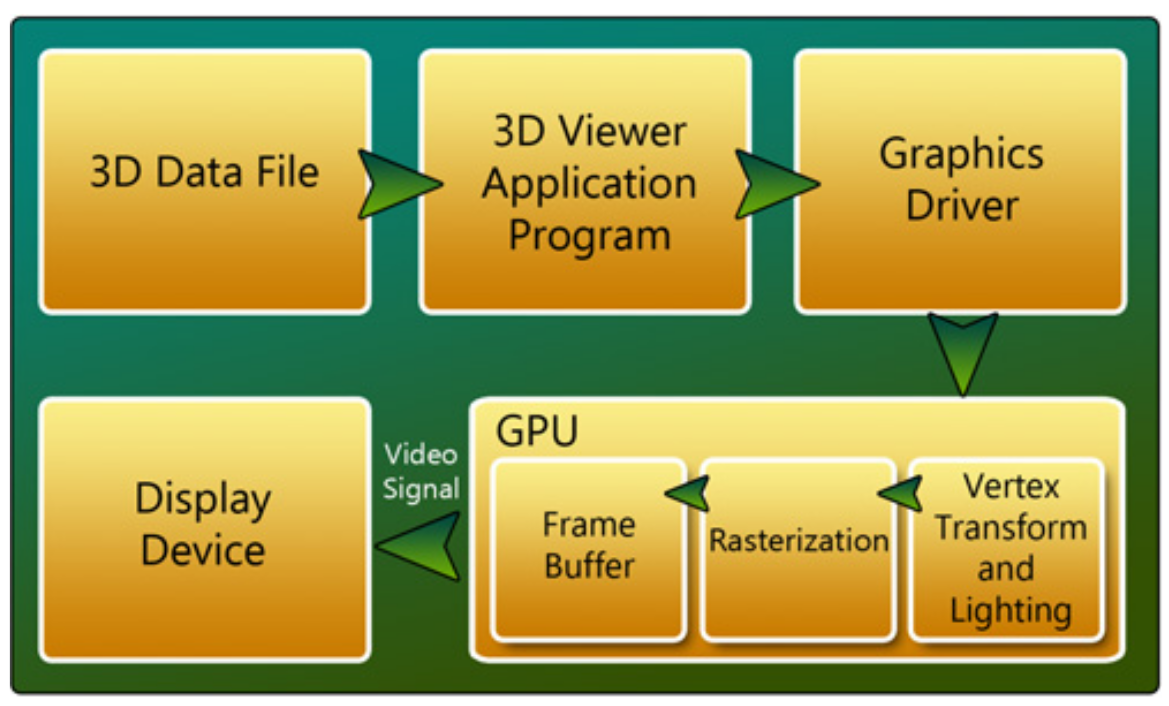
\includegraphics[scale=0.3]{images/pipeline}
	\caption{Schematizzazione della pipeline grafica.}
	\label{fig:pip}
\end{figure}
Obiettivo del mio periodo di ricerca (Novembre 2015-Luglio 2016) presso la \textit{University of Edinburgh} era quello progettare ed implementare un primo prototipo per risolvere il problema della visualizzazione interattiva all'interno di \textit{VELaSSCo}. La soluzione proposta è  quella dell'applicazione del offline rendering parallelo.
Durante il processo di rendering i dati RAW vengono trasformati  all'interno della pipeline grafica (Figura \ref{fig:pip}) fino ad arrivare in ultima istanza ad essere quello che è un sottoprodotto grafico direttamente visualizzabile dalle schede grafiche, il frame-buffer la cui  dimensione è relativamente piccola (decine di MB nel peggiori dei casi).
L'idea è quella che tutto il processing grafico avvenga in remoto direttamente sulle macchine che fanno HPC e che l'analista riceva solamente i framebuffers.
Queste idee sono state
La soluzione proposta è stata quella di:
\begin{itemize}
	\item progettare ed implementare un layer di rendering parallelo
	\item dotare la piattaforma di un numero di nodi dedicati al processing grafico (il cui numero è determinato in base al carico massimo del sistema, al numero di utenti connessi simultaneamente etc.)
	
\end{itemize}

Il processo di rendering può essere visto come un problema di ordinamento delle primitive grafiche sulla superificie dello schermo. In un renderer parallelo questo sorting richiede la ridistribuzione delle primitive tra tutti i processori perché la responsabilità per il rendering dello schermo è condivisa.
Esistono principalmente tre tipi di rendering parallelo, \textit{Sort First, Sort Middle} e \textit{Sort Last}; ognuno di essi differisce dagli altri per il momento in cui questa suddivisione avviene. Teoricamente essa può avvenire in qualunque istante durante l'esecuzione della pipeline grafica (Figure \ref{fig:sl} e \ref{fig:sfsm}).


\begin{figure}[!htbp]
	\centering
	\begin{minipage}{0.4\textwidth}
		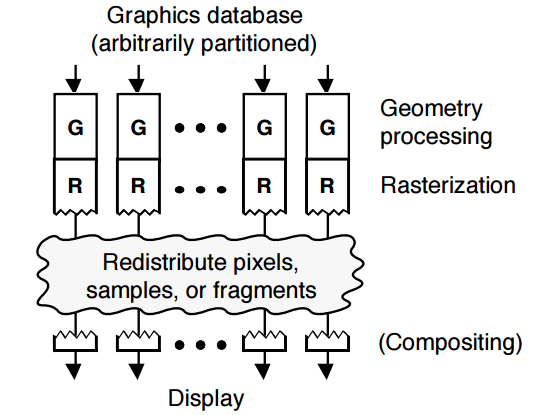
\includegraphics[scale=0.28]{images/sortlatst}
		\label{fig:sf}
	\end{minipage}
	\hfill
	\begin{minipage}{0.5\textwidth}
		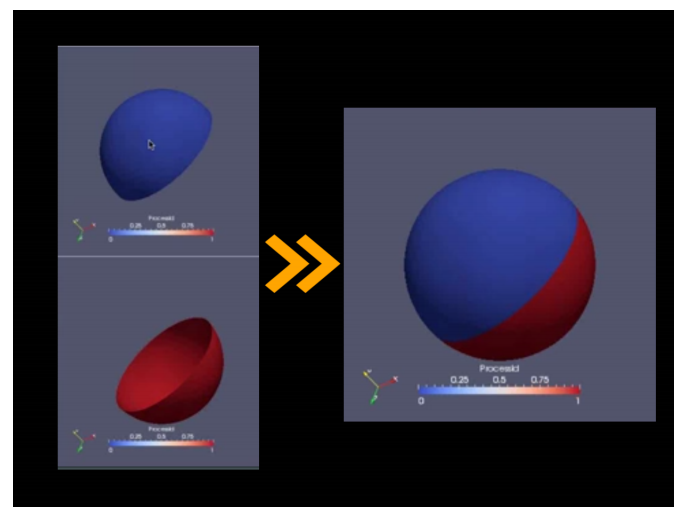
\includegraphics[scale=0.28]{images/sortlastex}
	\end{minipage}
	\caption{Sort-last. Esempio di composizione finale del framebuffer.}\label{fig:sl}
\end{figure}

Il prototipo sviluppato è di tipo sort-last, poiché questa strategia è l'unica che non suddivide le primitive in base alla porzione di schermo che modificano.
Il set di primitive grafiche viene suddiviso tra i processori secondo una policy che garantisce il load balancing (ogni processore può calcolare primitive che modificano qualunque parte dello schermo) e in fase di rastering tutti i risultati intermedi vengono \textit{ricomposti} a formare un unico framebuffer. La composizione avviene tenendo in considerazione lo z-buffer (Figura \ref{fig:sl}).

Il primo prototipo implementato ha mostrato ottimi risultati in termini di numero di primitive per secondo eseguite ed è in grado di effettuare il rendering di dati su schermi ad altissima risoluzione (schermi compositi). 



\begin{figure}[!htbp]
	\centering
	\begin{minipage}{0.4\textwidth}
		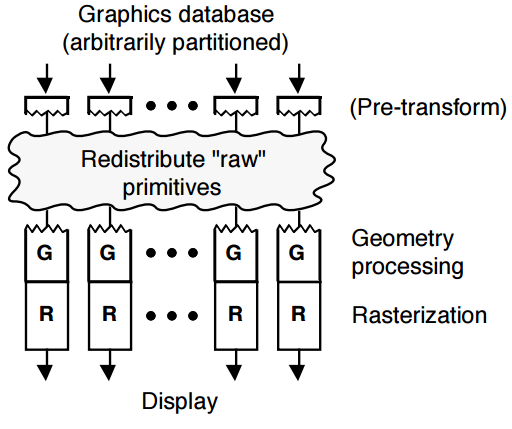
\includegraphics[scale=0.28]{images/sortfirst}      
		\label{fig:sf}
	\end{minipage}
	\hfill
	\begin{minipage}{0.4\textwidth}
		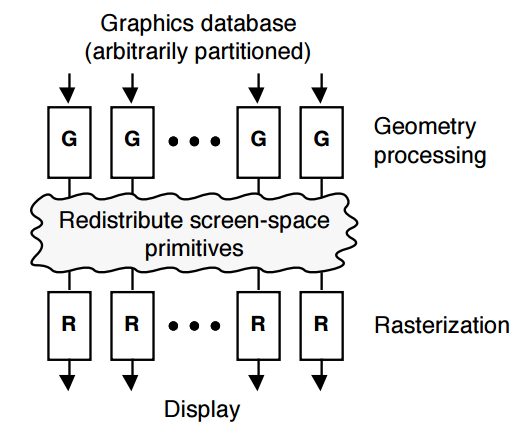
\includegraphics[scale=0.28]{images/sortmiddle}
		\label{fig:sm}
	\end{minipage}
	\caption{Sort first and Sort middle rendering.}\label{fig:sfsm}
\end{figure}


\subsection{Particle-like Objects Tracking}
\definecolor{myblue}{RGB}{80,80,160}
\definecolor{mygreen}{RGB}{80,160,80}
\begin{figure}[!htbp]
	\centering
	\begin{tikzpicture}[thick,
	every node/.style={draw,circle},
	fsnode/.style={fill=gray!30},
	ssnode/.style={fill=gray!90},
	every fit/.style={ellipse,inner sep=-2pt,text width=cm},
	->,shorten >= 3pt,shorten <= 3pt
	]
	
	% the vertices of Frame1
	\begin{scope}[start chain=going below,node distance=5mm, every node/.style={circle,minimum size=3.35em}]
	
	\node[fsnode,on chain,label=above:$\boldsymbol{M_{i}}$] (f0)  {$p^i_1$};
	\node[fsnode,on chain] (f1)  {$p^i_2$};
	
	\node[below of=f1,node distance=10,yshift=-10] {$\vdots$};
	
	\node[fsnode,on chain] (f2)  {$p^i_{j}$};
	\node[below of=f2,node distance=10,yshift=-10] {$\vdots$};
	\node[fsnode,on chain] (fl)  {$p^{i}_l$};
	\node[below of=fl,node distance=10,yshift=-10] {$\vdots$};
	
	\node[fsnode,on chain] (f3) {$p^i_n$};
	\end{scope}
	
	% the vertices of Frame1
	\begin{scope}[xshift=6cm,start chain=going below,auto, every node/.style={circle,minimum size=3.3em},node distance=5mm]
	
	\node[ssnode,on chain,label=above:$\boldsymbol{P_{i+1}}$] (s0)  {$p^{i+1}_1$};
	\node[ssnode,on chain] (s1)  {$p^{i+1}_2$};
	\node[draw=none,below of=s1,node distance=10,yshift=-10] {$\vdots$};
	
	\node[ssnode,on chain] (sk)  {$p^{i+1}_k$};
	\node[draw=none,below of=sk,node distance=10,yshift=-10] {$\vdots$};
	\node[ssnode,on chain] (s2)  {$p^{i+1}_{m-1}$};
	\node[ssnode,on chain] (s3)  {$p^{i+1}_m$};
	\end{scope}
	% the set U
	
	\node [myblue,draw=none] {};
	% the set V
	\node [mygreen,draw=none] {};
	\begin{scope}[every edge/.style={draw,thin}]
	% the edges
	\draw (f0) edge[red, thick, dashed]  (s3);
	\foreach \i in {0}
	\foreach \j in {0,1,2}
	\draw (f\i) edge  (s\j);
	
	
	\draw (f1) edge[red,thick, dashed]  (s0);
	\foreach \i in {1}
	\foreach \j in {1,2,3}
	\draw (f\i) edge  (s\j);
	
	\draw (f2) edge[red, thick,dashed]  (s1);
	\foreach \i in {2}
	\foreach \j in {0,2,3}
	\draw (f\i) edge  (s\j);
	
	\draw (f3) edge[red, thick,dashed]  (s2);
	\foreach \i in {3}
	\foreach \j in {1,3,0}
	\draw (f\i) edge  (s\j);

	\end{scope}
	
	\end{tikzpicture}
	\label{match}
\end{figure}
Il tracking di oggetti microscopici svolge un ruolo molto importante in molti ambiti scientifici per lo studio del movimento di particelle,  micro-sfere   e nanoparticelle. In particolare lo studio delle traiettorie che questi oggetti assumono è importante per calcolarne proprietà cinametiche e dinamiche. Vengono frequentemente utilizzate tecniche semi-automatiche per il tracking, ma questo approccio non è efficace quando il numero di particelle è grande.
Ho sviluppato quindi un software basato sul paradigma degli automi cellulari estesi (XCA) che è in grado di ricostruire le traiettorie di questo tipo di oggetti in modo automatico ed ho lavorato congiuntamente con alcuni ricercatori dell'istituto di BioEngineering dell'Università di Edimburgo per l'applicazione di questo software ad un caso di studio reale: il tracking del batterio \textit{B.subtilis} in un dispositivo microfiudico.

L'algoritmo sviluppato è in grado di produrre un set di traiettorie $ T_n = \{ t_i \}$  s.t.  $t_i=\{ c^i_k,c^i_{k+1},\ldots,c^i_l \} $ a partire da un insieme di input di particelle $P=P_1 \cup P_2 \cup \ldots \cup P_n$ e una funzione $\mathcal{D} :  P \times P \mapsto \mathbb{R}$, 
la funzione  \textit{distanza}.
$P_i = \{p^j_i \; | \; 1 \leq j\; \}$ sono tutte le particelle al tempo $i$ e ogni particella $p_i^j$ è definita da un centroide, un bounding box che ne descrive le proprietà geometriche e spaziali. 
$\mathcal{D}(p,q)$ misura quanto è probabile che  $p$ sia stata trasformata in $q$ dopo l'applicazione di zero o più trasformazioni geometriche (scaling, traslazione, rotazione, shearing etc.). 

L'algoritmo ad ogni step processa un frame $P_i$ ed un set di traiettorie parziali $M_i$ cercando di trovare un match ta le particelle in $P_i$ ed una traiettorie in $M_i$ e può essere ridotto ad una variante del problema dell'assegnamento in un grafo bipartito.
Più specificatamente l'algoritmo consiste nel trovare un matching di peso minimo (non necessariamente perfetto) in un grafo bipartito diretto e pesato $G=(V,E)$ dove $V={M_i} \cup P_i$ è il set di nodi ${M_i}, P_i$ sono le due partizioni, $E = {M_i} \times P_i$ t.c. $e \in E, \mathcal{D}(e) \in \mathbb{R}$ sia il peso dell'arco $e$.
Un matching valido deve soddisfare i seguenti constraints: 
\begin{equation}
\forall (u,v) \in S 
\left\{
\begin{array}{lr}
(w,x) \in S,\; v=x\Longleftrightarrow u=w\\
\mathcal{D}(u,v) = \min_{x \in V_2} \mathcal{D}(u,x)  \\
\nexists \: (w,v) \in E \: \mbox{s.t.} \: \mathcal{D}(w,v) < \mathcal{D}(u,v)
\end{array}
\right.
\label{matchConstraints}
\end{equation}
\begin{figure}[!htbp]
	\begin{minipage}[l]{0.5\textwidth}
		\centering
		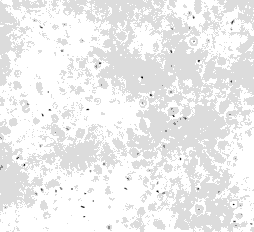
\includegraphics[width=5.5cm]{images/bacteriasmall}
		\caption{Immagine Raw di input. I Batteri appaio come cluster neri mentre grigio e bianco rappresentano rumore di fondo e abberazioni cromatiche dovute all'interazione della luce con il materiale del dispositivo microfluidico. } \label{AAA}
	\end{minipage}   
	\hfill{}
	\begin{minipage}[r]{0.5\textwidth}
		\centering
		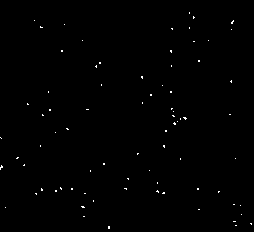
\includegraphics[width=5.5cm]{images/bacteriasmall_threshold}
		\caption{Immagine binaria ottenuta applicando filtri di threshold, constrast stretching e convoluzione gaussiana utilizzando il framework presentato. Rumore e backgraound sono stati eliminati, segmentando correttamente i batteri.} \label{BBB}
	\end{minipage}
\end{figure}
Se denotiamo  l'operatore di match utilizzando la seguente relazione di ricorrenza $  M_i \lozenge P_{i+1} = (T_{i+1},M_{i+1}) $, $M_0=P_0$, l'intera procedura può essere riscritta come $(T_n,M_n) = M_{n-1} \lozenge P_{n}=(((P_0 \lozenge P_1)\lozenge P_2) \lozenge \ldots \lozenge P_n)$.
Attualmente il lavoro che sto svolgendo è dimostrare che l'operatore $\lozenge $ è associativo, e sotto questa ipotesi la medesima procedura è immediatamente parallelizzabile utilizzando il paradigma della parallel reduction.

La Figura \ref{match} mostra un'applicazione dell'operatore $\lozenge$ al frame $P_{i+1}$ composto da $m$ particles. Le linee rosse tratteggiate mostrano la soluzione $S$.
Supponiamo ad esempio che esista una traiettoria in $M_i$, $t_*=p^s_a \leadsto p^i_1$ . Essa verrà ulteriormente allungata dal match trovato da $\lozenge$ con la particella $p^{i+1}_m$ diventando $t=p^s_a \leadsto p^i_1 \to p^{i+1}_m$.

Un framework basato sugli automi cellulari estesi che è in grado di effettuare operazioni di image processing su dati $n$-dimensionali come ad esempio la convoluzioni è stato sviluppato. Questo framework è intrinsecamente parallelo e può essere eseguito su diverse architetture parallele (una versione per macchine a memoria condivisa è già disponibile). Un esempio di utilizzo di tale framework è dato dalle Figure \ref{AAA} e \ref{BBB}.

I risultati ottenuti sono molto promettenti in quanto siamo stato in grado di calcolare alcuni parametri riguardanti il moto del batterio \textit{B. subtilis}, come il tempo di \textit{tumble} medio e la velocità di \textit{run}. 
Tutti i risultati sono in accordo con i valori standard trovati in letteratura, a conferma che le traiettorie sono ricostruite con buona precisione (Figura \ref{fig:res}).

\begin{figure}[!htbp]
	\begin{center}
		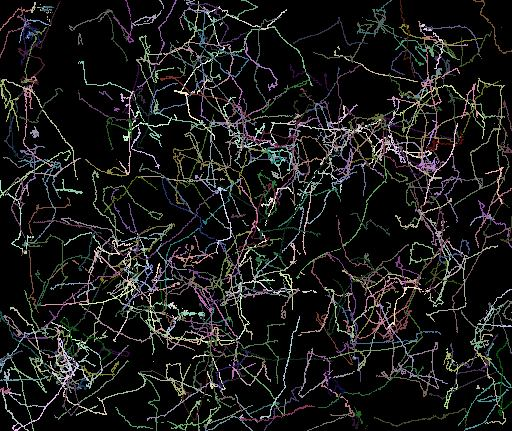
\includegraphics[scale=0.75]{images/result.png}
		\caption{Traiettorie traccate utilizzando un filmato time-lapse di 4100 frames. Per rendere più chiara l'immagine un colore random è associato ad ogni traiettoria.}\label{fig:res}
	\end{center}
\end{figure}


\part{Attività formative e di ricerca -  \RNum{3} anno}

\section{Corsi e Seminari}
\begin{itemize}
	\item \textbf{UKMAC 2017}, \textit{UK Manycore Developer Conference}, 11 Luglio 2017, University of Warwick
\end{itemize}

\section{Didattica}
\begin{description}
\item [\textbf{Esercitatore}] del corso di\textit{ Interfacce Grafiche e Programmazione ad Eventi} del CdL in \textit{Informatica}, \textit{Dipartimento di Matematica e Informatica}, UNICAL. \textbf{Periodo}: \textit{Marzo 2017 - Settembre 2017}
\end{description}

\section{Visiting presso altre università}
\begin{description}
	\item [da Giugno 2017 a Agosto 2017] presso il \textit{Department of Computer Science, University of Warwick (UK)} sotto la supervisione del Prof. \textit{Gihan R. Mudalige}.
\end{description}


\section{Pubblicazioni}
\begin{itemize}
	\item  Donato D'Ambrosio, Alessio De Rango, Marco Oliverio, Davide Spataro,
	William Spataro, Rocco Rongo, Giuseppe Mendicino, Alfonso Senatore:
	\textbf{The Open Computing Abstraction Layer for Extended Cellular
	Automata and the Finite Di fferences Method}, accepted with revisions to
	the \textit{ISI/SCOPUS Journal of Parallel and Distributed Computing (ISSN:
	0743-7315)}.

\item Donato D'Ambrosio, Alessio De Rango, Davide Spataro, Rocco Rongo,
William Spataro: Applications of the OpenCAL scientific library in
the context of CFD: \textbf{Applications of the \texttt{OpenCAL} scientific library to debris flows}, \textit{2017 IEEE 14th
International Conference on Networking, Sensing and Control (ICNSC)}

\item A. De Rango, D. Spataro, D. D’Ambrosio, R. Rongo, W. Spataro, \textbf{Fast
Lava Risk Assessment by Multi-GPU}, accepted at the \textbf{26th Euromicro
International Conference on Parallel, and Network-Based Computing
2018}, \textit{Cambridge (UK), March 21-23, 2018}

\end{itemize}


\section{Attività di Ricerca}
Durante il mio \RNum{3} anno di dottorato mi sono occupato principalmente di concludere, ottimizzare e testare il lavoro iniziato negli anno precedenti sulla librarie \texttt{OpenCAL}. La librerie si dimostra in grado di produrre implementazioni parallele di una classe di modelli numerici a griglia regolare, utilizzando un formalismo che nasconde sia i dettagli architetturali tecnici dell'hardware sul quale essi sono eseguiti che la complessità intrinseca del parallelismo. La libreria è stata testata su tre modelli differenti per caratteristiche e requirements computazionali. Tre benchmark sono stati adottati:
\begin{enumerate}
	\item Julia Set: \textbf{compute bound}
	\item Convolutional Filter:\textbf{memory/bandiwidth bound}
	\item sciddicaT: \textbf{memory e compute bound}
\end{enumerate} 
La sezione \ref{sec:convolutional_filters} mostra un esempio di implementazione di un semplice filtro convoluzionale (esempiodi memory bound application), \textit{Sobel}, in \texttt{OpenCAL} e i relativi risultati di performance ottenuti.

\subsection{Convolutional Filters}
\label{sec:convolutional_filters}
La convoluzione di un immagine può essere espressa in modo generico mediante la seguente formula:
\begin{equation}
f'_{ij} = \sum_{i'=0}^n (\sum_{j'i'=0}^m f_{(i+i')(j+j')}\times d_{ij})
\label{eq:convolution}
\end{equation}
dover 
\begin{itemize}
	\item $m,n$ sono le dimensioni verticali ed orizzonatali del kernel
	\item $f_{ij}$ e $f'_{ij}$ sono rispettivamente il vecchio ed il nuovo valore della cella alla posizione $(i,j)$,
	\item $d_{ij}$ è il valore del kernel alla posizione $(i,j)$ 
\end{itemize}
\begin{figure}[!htb]
	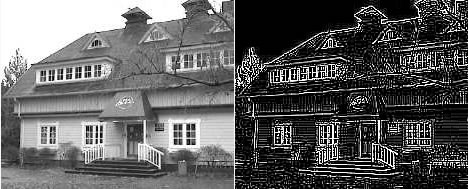
\includegraphics[width=\linewidth]{./images/sobel_example}
	
	\caption{Esempio dell'applicazione del filtro \textit{Sobel} implementato in \texttt{OpenCAL}. }
	\label{fig:sobel}
\end{figure}

Il filtro di Sobel è facilmente implementabile in \texttt{OpenCAL} seguendo gli step che seguono::
\begin{enumerate}
	\item L'immagine viene decomposta nei canali di colore rosso, verde e blu, e ognuno di esso è letto in un sottostato di tipo short.
	\item Un \textit{cluster} file viene definito il quale specifica (si veda Listato \ref{code:sobel_cluster_file}) come il dominio deve essere diviso tra le risorse computazionali a disposizione.
	\item Il codice che implementa l'applicazione di un kernel (si veda Listato \ref{code:sobel_kernel}) a un signolo punto del dominio viene specificato dal programmatore e automaticamente eseguito in parallelo su tutto il dominio. Se un device necessita di dati che sono stati assegnati ad un altro device, questi vengono automaticamente trasferiti in maniera trasparente, anche quando essi sono fisicamente installati su nodi separati (in quel caso attraverso anche una comunicazione MPI).
\end{enumerate}
\begin{figure}
	\centering
	\caption{Sobel Scaling}
	\label{fig:sobel_scaling}
	\includegraphics[width=0.6\textwidth]{../plots/sobel_scaling}
\end{figure}
\lstset{language=[OpenCL]C,frame=tb,
	caption=Adopted cluster file for the Sobel filtering example. The image is decomposed equally among 3 devices. , 
	basicstyle=\footnotesize\ttfamily,
	label={code:sobel_cluster_file}
}
\begin{lstlisting}[float]
10800 21600
1
192.168.1.111 3
0 0 3600
0 1 3600
0 2 3600
\end{lstlisting}
Figure \ref{fig:sobel_scaling} mostra come il filtro Sobel scala al crescere del numero delle GPU utilizzate. Si noti come schede diversi tipi di schede (marca ed architettura) possono essere utilizzate allo stesso momento.
La  Figura \ref{fig:sobel_2nodes_performance} mostra lo stesso codice eseguito su due nodi differenti. Come si può vedere anche in questo caso, in cui una comunicazione via rete è necessaria, buone performance sono ottenute, con un picco di $\approx 81\times$ quando tre devices sono utilizzati in modo concorrente.
La libreria supporta anche architetture distributed memory e,la Figura \ref{fig:sobel_2nodes_k40+980-K20+980} mostra tempi e speedups per un esecuzione su due nodi, ognuno dei quali equipaggiato con due acceleratori (per un totale di $4$). 
In questo caso è stato ottenuto un miglioramento di circa $\apoprox 22 \times$ e $\approx 103$ rispetto ad un esecuzione su $3$ GPU su un singolo nodo (si veda Figura \ref{fig:sobel_scaling}) e l'esecuzione \textbf{seriale} su un singolo core.
\begin{figure}[!htb]
	\minipage{1.0\textwidth}
	\begin{subfigure}{1.0\textwidth}
		\caption{Performance on $2$ nodes and $2$ GPUs: \texttt{NVIDIA K40}(\textit{node 1}) and $1$ \texttt{GTX980}(\textit{node 2}).}
		\label{fig:sobel_2nodes_k40_980}
		\includegraphics[width=1.0\textwidth]{../plots/sobel_2nodes_k40_980}
		
	\end{subfigure}        
	\endminipage \hfill
	\minipage{1.0\textwidth}
	\vspace{5mm}
	\begin{subfigure}{1.0\textwidth}
		\includegraphics[width=1.0\textwidth]{../plots/sobel_2nodes_k40+980-K20+980}
		\caption{Performance on $2$ nodes each with $2$ GPUs.}
		\label{fig:sobel_2nodes_k40+980-K20+980}
	\end{subfigure}
	\endminipage\hfill
	\caption[\textit{Sobel} filter benchmark performance metrics on two nodes.]{\textit{Sobel} filter benchmark performance metrics on two Ethernet interconnected nodes. (a) reefers to the case where node 1 is equipped with $1$ $K40$ and node 2 with a $GTX980$. (b) to the case where \textit{node 1} uses a $K40$ and a $GTX980$ while \textit{node 2} a $K20$ and a $GTX980$. Time in red (lower is better), speed-up in blue (higher is better).}
	\label{fig:sobel_2nodes_performance}
\end{figure}
\begin{minipage}{1.0\textwidth}


\lstset{language=[OpenCL]C,frame=tb,
	caption=\texttt{OpenCAL} Sobel edge detection filter kernel., 
	label={code:sobel_kernel}, 
	basicstyle=\footnotesize\ttfamily,
	keywordstyle=\color{blue}\ttfamily,
	stringstyle=\color{red}\ttfamily,
	commentstyle=\color{green}\ttfamily,
	backgroundcolor=\color{light-gray}, 
	numbers=left,numbersep=3pt, 
	numberstyle=\tiny\ttfamily\color{gray}
	%    numberstyle=\tiny
}
\begin{lstlisting}
__kernel void sobel2D_transitionFunction(__CALCL_MODEL_2D) {
	calclThreadCheck2D();
	int i = calclGlobalRow() + borderSize;
	int j = calclGlobalColumn();
	int KX[3][3] = {{-1, 0, 1}, {-2, 0, 2}, {-1, 0, 1}};
	int KY[3][3] = {{1, 2, 1}, {0, 0, 0}, {-1, -2, -1}};
	int Gx, Gy, n, k, k1;
	Gx = Gy = n = 0;
	if (j > 0 && j < calclGetColumns() - 1)
		for (k = -1; k <= 1; k++)
			for (k1 = -1; k1 <= 1; k1++) {
				Gx += calclGet2Di(MODEL_2D, DEVICE_Q_red, i + k, j + k1) *
				KX[k + 1][k1 + 1];
				Gy += calclGet2Di(MODEL_2D, DEVICE_Q_red, i + k, j + k1) *
				KY[k + 1][k1 + 1];
			}
	const int P = sqrt(Gx * Gx + Gy * Gy);
	// set new pixel color for red channel
	calclSet2Di(MODEL_2D, DEVICE_Q_red, i, j, P);
	return;
}
\end{lstlisting}
\end{minipage}

	
\end{document}
